\documentclass[12pt]{article}
\input{.house-style/preamble.tex}
\usepackage{float}
\usepackage{tikz}
\usetikzlibrary{arrows.meta, positioning}
\hypersetup{
  pdftitle={From Aggregate Scores to Warranted Inference in AGI Evaluation},
  pdfkeywords={AGI evaluation, validity, projectibility, tail risk, generalization}
}
\setlength{\headheight}{14pt}
\setlength{\emergencystretch}{1.5em}

\newcommand{\ins}{\mathrm{INS}}
\newcommand{\wtd}{\mathrm{WTD}}
\newcommand{\wtl}{\mathrm{WTL}}

\title{From Aggregate Scores to Warranted Inference\\in AGI Evaluation}
\author{Brett Reynolds \orcidlink{0000-0003-0073-7195}\thanks{I used ChatGPT 5, Claude Sonnet 4.5, and Gemini Pro 2.5 extensively in drafting and revising this paper. I reviewed, edited, and approved all the material and take full responsibility for the final text and conclusions. \href{mailto:brett.reynolds@humber.ca}{brett.reynolds@humber.ca}}\\
Humber Polytechnic \& University of Toronto}
\date{}

\begin{document}

\maketitle

\begin{abstract}
Multidomain test batteries are increasingly used to judge how close AI systems are to general intelligence, and a single score is then read as evidence about tasks, users, systems, and future versions the test never covered. A precise, repeatable score doesn't by itself support those wider claims. Standardizing a test fixes what it measures narrowly, and averaging over items hides how a system behaves: one mean is consistent with no change, with improvements and failures that cancel, and with a stable core of serious errors.

This paper adapts validity theory from psychological measurement, where what's assessed is the argument for a particular interpretation and use of a test's scores, not the test itself. A claim about another task type, user group, system build, or future period is a new inference carrying its own evidential burden. I call the standing of such a claim its \term{projectibility}, after Goodman. Evaluators should state what was observed, identify the unobserved cases to which the result is being extended, and test the differences between the two that could change the result.

A reanalysis of 32 released model--benchmark comparisons, and simulations with known answers, show that a stable average can hide large offsetting shifts and persistent severe failures, and that different estimators of these effects answer different questions. They don't show that any score predicts untested performance. Because no developer can foresee every use, the burden divides: developers report the exact systems, items, prompts, scoring rules, and variations they tested; deployers sample their own tasks, score the failures that matter there, compare available policies, and monitor what reaches users.
\end{abstract}

\noindent\textbf{Keywords:} AGI evaluation; validity; projectibility; tail risk; generalization

\section{The Inferential Overreach of AGI Scores}\label{sec:problem}

Multidomain evaluations are routinely read as evidence for inferences or decisions beyond their observed results. Combining domain scores into a total discards detail. The problem is that evaluators rarely check whether the discarded detail matters to the inference or decision.

This paper adapts validity theory from educational and psychological measurement. Its central move is to treat validity not as a property of a test in isolation but as the strength of the argument for a proposed interpretation of its scores and use of them \citep{messick1995Validity,kane2013validating}. A score may be precise and repeatable for a restricted set of observations while providing weak evidence for a broader claim.

Goodman's new riddle of induction isolates the underlying problem. Suppose that every emerald examined before a specified time \(t\) has been green. Those observations fit the familiar hypothesis that all emeralds are green.

Now define a second predicate. An object is \mention{grue} if it was examined before \(t\) and is green, or if it wasn't so examined and is blue. The same observations fit the hypothesis that all emeralds are grue. The two hypotheses agree about every emerald observed so far but disagree about an emerald first examined after \(t\): the green hypothesis predicts a green emerald; the grue hypothesis predicts a blue one. The riddle asks why the first is \term{projectible}, or fit for projection beyond the observed cases, while the second isn't \citep[74--80]{goodman1983}.

Goodman answers the riddle by appealing to the history of inductive practice, not to a better fit with the observed emeralds: green and grue fit them equally well. \mention{Green} has repeatedly figured in past projections; \mention{grue} hasn't. He calls this history \term{entrenchment} and uses it to distinguish otherwise equally supported predicates \citep[84--86, 93--98]{goodman1983}. \Textcite[136--141]{boyd1991} places more weight on empirically revisable background theory and, for inductive or explanatory categories, causal structure. I borrow the question and vocabulary of projectibility without treating either entrenchment or causal structure as a sufficient criterion of warrant.

The analogous question for AI benchmarks is whether success on scored items warrants a broader claim. Observed successes may fit both the claim that a system performs well across a domain and the rival claim that it performs well only on tasks sharing the tested formats or contexts. The claims agree on the scored items and diverge on the cases that motivate broader evaluation. I adapt \term{projectibility} to name the degree of warrant for a specified claim that extends an interpretation, prediction, or explanation from the observed evaluation to a bounded target.

A running example fixes the source and target. Suppose a developer reports a high legal-reasoning score from a battery whose items present a question with a fixed set of materials and mark the model's answer against a reference response. An employment-law group is considering a different object: an assistant that receives a lawyer's research question, searches a live legal database, and drafts a one-page memo with linked authorities. The group initially limits the use to Ontario wrongful-dismissal files asking about termination clauses or reasonable notice. Each memo must identify the issue, cite the current controlling authorities, link each legal proposition to a passage that supports it, and be checked by a lawyer before it leaves the firm. The battery observes none of the search, source-updating, citation, or review steps.

An independent evaluation of leading commercial legal-research assistants found them fabricating authority between 17\% and 33\% of the time, against vendor assurances of hallucination-free citation \citep{magesh2025legalhallucination}. That study doesn't predict the performance of this assistant, but it identifies something the firm must count rather than hide inside an overall quality score. The firm can draw research requests from closed files that meet the inclusion rule, keep every request from the same client file in one data split, and have two lawyers who supervise these file types independently prepare the required authorities and propositions before they see the assistant's outputs, resolving disagreements before scoring begins. Blinded reviewers can then record whether each citation resolves, whether the cited passage supports the proposition, whether a controlling authority was omitted, which defects the assigned lawyer caught, and how long review took. Those observations could support a claim about the frozen assistant and review procedure on the request types sampled. They couldn't turn the developer's battery score into evidence of broad legal capability. The battery result is one source observation; the claim about reviewed memos on eligible research requests is the target claim.

The source score comes from a standardized evaluation, which fixes prompts, scoring, and conditions so that repeated evaluation answers a stable question. Standardization also narrows the \term{evaluation universe}: the tasks, prompts, scoring rules, and conditions represented by the score.

\begin{figure}[tbp]
\centering
\footnotesize
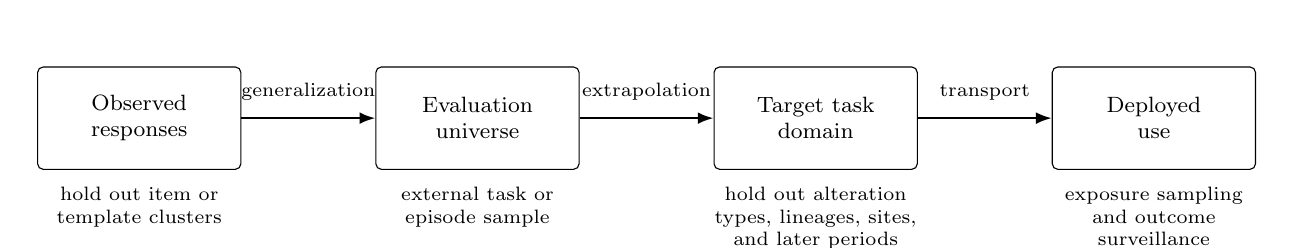
\begin{tikzpicture}[
  node distance=6mm,
  box/.style={draw, rounded corners=2pt, align=center, inner sep=4pt,
              text width=23mm, minimum height=13mm, font=\footnotesize},
  flow/.style={-{Latex[length=2mm]}, thick},
  lab/.style={align=center, font=\scriptsize, text width=25mm}
]
\node[box] (obs) {Observed\\responses};
\node[box, right=17mm of obs] (uni) {Evaluation\\universe};
\node[box, right=17mm of uni] (dom) {Target task\\domain};
\node[box, right=17mm of dom] (dep) {Deployed\\use};

\draw[flow] (obs) -- node[lab, above=1mm] {generalization} (uni);
\draw[flow] (uni) -- node[lab, above=1mm] {extrapolation} (dom);
\draw[flow] (dom) -- node[lab, above=1mm] {transport} (dep);

\node[lab, below=1mm of obs.south, text width=26mm] {hold out item or template clusters};
\node[lab, below=1mm of uni.south, text width=26mm] {external task or episode sample};
\node[lab, below=1mm of dom.south, text width=26mm] {hold out alteration types, lineages, sites, and later periods};
\node[lab, below=1mm of dep.south, text width=26mm] {exposure sampling and outcome surveillance};
\end{tikzpicture}
\caption{Where a score has to travel, and what answers each step. Each arrow is a separate claim with its own evidence, and warrant for one doesn't carry to the next. The lower row names the design that addresses the step above it; Table~\ref{tab:projection_relations} gives the full set of relations.}\label{fig:where_scores_travel}
\end{figure}

\Textcite[22--25]{kane2013validating} distinguishes two moves: generalizing from observed scores to a test's standardized universe and extrapolating from that universe to a broader target domain. Figure~\ref{fig:where_scores_travel} places those moves in the longer chain the running example needs. \Textcite[132--135]{brennan2001generalizability} shows why the distinction matters: a feature held fixed in the restricted universe may vary in the broader one, so standardization can raise precision within the former while weakening extrapolation to the latter. More observations from the narrowed universe leave systematic underrepresentation of the target intact.

Underrepresentation of the target is one inferential gap. Aggregation creates another even within a fixed evaluation universe. \Textcite[2, 4--6]{zhang2026illusionRobustness} provide a controlled example: they add task-irrelevant context to benchmark items and find that aggregate accuracy often moves little even when item-level response probabilities move in opposite directions. After subtracting the change expected from repeated baseline sampling alone, their estimates reach 13.6\% for mean absolute item change and 53.2\% for worst-decile degradation. The affected examples are also largely model-specific: on MMLU-Pro the mean cross-model correlation of per-item change is .00, and the mean Jaccard overlap of the most-affected decile is .09.

A stable mean is compatible with unchanged items, balanced improvements and degradations, deterioration concentrated in a tail, or a persistent set of serious failures. Those states may support different predictions and decisions. The declared target identifies distinctions that may need to be preserved; matched evidence determines which earn a place in a target-specific report. Figure~\ref{fig:stable_mean_states} sets the four side by side.

\begin{figure}[htbp]
\centering
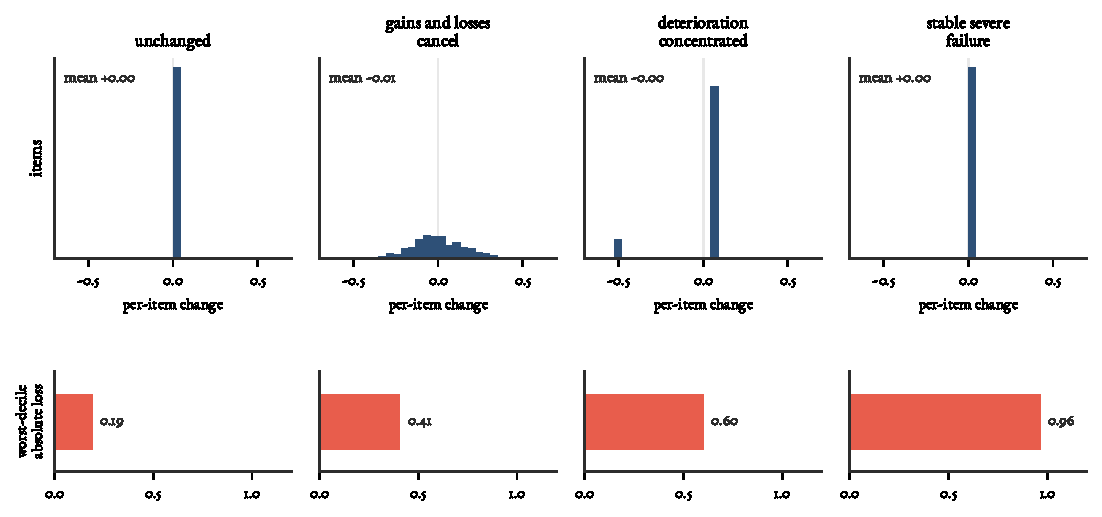
\includegraphics[width=0.96\linewidth]{analysis/outputs/stable_mean_states.pdf}
\caption{Four item-level states behind one stable mean, constructed for illustration rather than measured. The top row gives the distribution of per-item change; all four have the same near-zero mean. The bottom row gives the resulting worst-decile absolute loss. The first and fourth columns are indistinguishable in the top row and differ by .19 against .96 in the bottom one, which is why a change statistic can't stand in for an absolute risk measure.}\label{fig:stable_mean_states}
\end{figure}

The gap between the standardized evaluation universe and the intended target is widest when the target is general capability itself, since no target reaches further beyond a fixed set of tested cases. \Textcite{raji2021whole} argue that broad benchmark claims routinely outrun the contextual tasks used to construct them. \Textcite{hendrycks2025agi} propose the most developed framework aimed squarely at that target, evaluating AGI across ten cognitive domains guided by Cattell--Horn--Carroll (CHC) theory, a hierarchical account of human cognitive abilities inferred from test-score correlations. They themselves warn that a total can conceal bottleneck failures, and recommend reporting the domain profile, the vector of domain scores, alongside it.

The profile preserves distinctions that a total erases, but it still compresses item changes and tails, and its domain structure may not transfer across systems (Section~\ref{ssec:chc_scope}). A score is an indicator, not the capability or attribute it's meant to represent; validity theory calls the represented capability or attribute the \term{construct} \citep[742]{messick1995Validity}. Neither total nor profile establishes which inferences the ten-domain framework supports beyond its construction; a broader construct interpretation requires an additional argument \citep[24]{kane2013validating}.

Before an aggregate is interpreted as a measure or used in a decision, three separate questions arise: whether its components share a meaningful scale (commensurability), whether the tradeoffs it permits are acceptable (compensability), and whether the resulting score supports the declared target inference (projectibility).

The AGI label imports a claim of generality that no finite test set exhausts. A battery may stipulatively define an AGI index and report it accurately; the open-ended claim begins when that index is read as evidence of general capability beyond its construction domain, which coverage alone can't validate. The developer's broad-capability claim is of that kind, and no finite local study can settle it. The firm can ask a smaller question: whether one frozen assistant, used with line-by-line verification that every citation resolves and supports the accompanying proposition, produces reviewed memos meeting stated criteria for the two eligible kinds of employment-law request. Answering that question requires new observations from those requests; it doesn't enlarge the meaning of the battery score. Aggregates can describe their construction samples. Claims about other work require evidence from that work or a defensible account of why the relevant differences won't matter.

Two adjacent proposals share the diagnosis and divide the labour differently. \Textcite{liu2024ecbd} adapt evidence-centred design from educational assessment, formalizing benchmark construction into five modules and requiring designers to describe, justify, and support each choice, with case studies of three widely used language benchmarks (BoolQ, SuperGLUE, and HELM). Their subject is the evidence a benchmark collects about the capabilities it declares; movement beyond the benchmark isn't their topic. \Textcite{binetteReiter2024estimands} adapt the estimands framework of the clinical-trials guidelines, characterizing an estimand by a metric, a scope or population, a data-acquisition strategy, and an aggregation rule, after which an estimator and its uncertainty are chosen. They do press how performance generalizes beyond a benchmark, showing how cross-validation and benchmark composition can mislead. What differs here is the organizing unit. Theirs is an estimand specified by metric, population, data acquisition, and aggregation. This paper's is an inferential chain (Figure~\ref{fig:where_scores_travel}) whose links may call for different estimands, different holdout units, and different parties to supply the evidence.

This paper uses \term{transport} for a claim's movement across contexts, systems, sites, or times. In causal inference, transportability is a narrower and more demanding notion. \Textcite{pearlBareinboim2014transportability} represent domain differences in selection diagrams and give conditions under which a causal relation in the target is uniquely computable from the source's observational and interventional distributions together with the target's observational distribution (their Definition 5). The sense used here is broader and non-causal, and claims none of those identification guarantees.

What this paper adds to those accounts is a combination: projectibility assessed claim by claim, from specified source observations to bounded targets, rather than for an evaluation as a whole; the assumptions required for each projection exposed and tested against the differences they concern; behavioural-change quantities separated from target-conditioned loss; and evidential responsibility divided between developer and deployer. Two supported projections may be combined only when the cases reached by the first are the cases sampled by the second, their assumptions are compatible, and their dependence and uncertainty are carried through.

This paper makes three linked contributions. First, it turns claims beyond the observed evaluation into explicit, separately testable projections to bounded targets and assigns responsibility for their evidence. Second, it shows why several kinds of behavioural change and target-conditioned risk can't generally substitute for one another. Third, it distinguishes the evidence a developer can publish about a reference evaluation from the task samples, review records, policy comparisons, and outcome monitoring a deployer must supply for a particular use. The reanalysis and simulations test the second contribution's statistical machinery; they don't validate an external deployment projection.

\section{Projectibility within a Validity Argument}\label{sec:projection}

Validity theory supplies the method used here. \Textcite[741]{messick1995Validity} uses \term{score} broadly, for any qualitative or quantitative summary of observed regularities in people, groups, environments, objects, or institutions. Kane's argument-based approach writes a proposed interpretation and use as a sequence of claims and assumptions, then asks whether each is coherent, necessary, and supported. The more ambitious the interpretation or use, the more evidence that sequence requires \citep[1--3]{kane2013validating}. In the example, the objects have to be kept separate: the model that answered supplied-text benchmark questions, the later model connected to a legal database, the draft that system produced, and the memo after a lawyer checked it. Evidence about one isn't automatically evidence about the next.

A projection extends an interpretation, prediction, or explanation from specified observations to cases not observed in the source study. I use \term{projectibility} for the degree of warrant for that extension. A high score and a statement that the cases are similar supply no such warrant by themselves. The evaluator has to name differences that could change the result and investigate them: sample cases from the proposed range, vary features suspected of causing failure, and state the revisable background knowledge that makes those features relevant. For the legal assistant, the obvious differences are live retrieval, changing authority, open-ended drafting, citation verification, lawyer review, and a later model build.

The battery supports a claim about answers to its supplied-text questions. The firm's study would address a different claim. It would run the frozen assistant on held-out termination-clause and reasonable-notice requests, score the draft before review, let the assigned lawyer verify every citation and supporting passage under the written review instructions, and score the final memo again. A result from that study would extend from the sampled requests to other requests admitted by the same inclusion rule; it wouldn't make the battery score general. It might support mandatory-review use for those two request types while leaving tax research, another province, or unreviewed drafting unsupported. Projectibility is therefore graded and claim-relative. A \term{projectibility audit} is the record of this reasoning: the benchmark observations, the exact claim about the two request types, each difference between them, the evidence used to examine that difference, and the result that would narrow or defeat the claim.

For confirmatory use, the firm fixes the claim and the support, defeat, and inconclusive conditions before opening the final holdout. It records the exact model build, legal-database snapshot, system prompt, drafting template, and review instructions; defines which logged research requests qualify; groups all requests from one client file in the same split; defines each scored defect; and fixes the tail fraction and decision tolerance. Closed files used to write prompts, choose the rubric, or decide which defects matter remain development data. Confirmation uses a later untouched block of eligible files. Adding more supplied-text benchmark questions could strengthen a claim about that question format, but it wouldn't test live retrieval, current authority, linked citations, or the specified line-by-line lawyer review.

Prospective declaration narrows discretion without eliminating it. Reviewers may disagree about whether a cited passage supports a proposition, one output may contain two requests, and results may differ between termination-clause and reasonable-notice research. The analyst still has choices about adjudication, whether to pool the two request types, how to estimate a tail, and which experience groups of lawyers to examine. Because those choices can alter the estimate or conclusion, the audit records them and treats unplanned alternatives as exploratory rather than as independent confirmations \citep{GelmanLoken2013}.

The audit also keeps four things distinct. The claim might be that reviewed memos on eligible requests stay below a stated defect tolerance. The observations are the held-out drafts, review logs, and rescored final memos. The empirical regularity is the estimated defect distribution. A proposed explanation might be that the database retrieves every controlling case and line-by-line review catches unsupported propositions. The observations may support the prediction without establishing that explanation; retrieval logs may support the explanation for past cases without showing that it survives another request type or model build. Projectibility concerns the warrant for the projected claim, not whether a complete causal account has been found.

The authorization decision adds a separate layer. Even a well-supported estimate of defects has to be compared with feasible policies: no assistant, use only to suggest search terms, drafting with line-by-line citation verification, or drafting with a lighter check. The firm must weigh lawyer time, missed or unsupported authority, confidentiality, and the possibility that an error reaches a client or court. Those values enter before the final choice as well: classifying an unresolvable citation as a red-line defect, rather than one error among several that can average out, is already a value-laden scoring decision \citep[747--749]{messick1995Validity}.

Projectibility concerns only the inferences that extend beyond observed cases in the larger validity argument. \Textcite[741--747]{messick1995Validity} asks five further questions: whether the benchmark content represents what the score is said to cover, whether the responses engage the processes named in that interpretation, whether the scoring fits the construct, whether the score relates to external criteria, and whether the consequences bear on the proposed use. The firm's holdout can't answer all five. Nor can one holdout answer every extension. Generalizing from sampled closed files to later eligible requests requires new requests selected by the same rule; moving from employment law to tax requires tax tasks; replacing the model or retrieval index requires a new system test; and claiming stable performance over the next year requires chronological evidence.

System transport requires one further term. Here, \term{lineage} denotes systems (the developer's benchmarked model, its later releases, and the firm's assistant built on one of them) whose results may be dependent because they share training runs, distillation, retrieval components, evaluation data, or other declared provenance. Twenty outputs from one build are twenty response replicates, not twenty systems. A new product label may still denote a fine-tune of the same base model or the same retrieval stack, so its success isn't an independent confirmation. The firm often can't establish the dependence because training overlap and shared components are proprietary. Any analysis that treats successive builds as independent therefore has to state and defend that assumption.

Table~\ref{tab:projection_relations} distinguishes eight inferential relations and then separates them from decision use. Each row poses a different evidential question within one interpretation-and-use argument.

\begin{table}[tbp]
\centering\scriptsize
\renewcommand{\arraystretch}{0.92}
\caption{Inferential relations, decision use, and especially relevant evidence.}\label{tab:projection_relations}
\begin{tabular}{@{}>{\raggedright\arraybackslash}p{0.25\linewidth}
                    >{\raggedright\arraybackslash}p{0.29\linewidth}
                    >{\raggedright\arraybackslash}p{0.37\linewidth}@{}}
\toprule
Claim or use & Declared range & Especially relevant evidence \\
\midrule
Observed responses to further responses of the same kind (generalization) & New items, template clusters, or repeated outputs generated under the test rules & Sample from the stated item-generating process; keep whole templates out of training and tuning; repeat outputs only to estimate within-item variation \\
Benchmark tasks to the proposed work (extrapolation) & For example, supplied-text legal questions to logged research requests requiring live retrieval and a cited memo & Sample external requests by a written inclusion rule, prepare reference answers independently, and score the outputs against them \\
One input condition to another & For example, a clean retrieval corpus to one containing irrelevant but topically similar cases, reordered documents, or paraphrased instructions & Keep an entire alteration type out of tuning and test it on held-out requests \\
One system to another & A different model build, retrieval index, prompt stack, or dependency lineage & Evaluate the new configuration on untouched cases; don't count repeated outputs or closely related builds as independent systems \\
One team or site to another & Different lawyers, review instructions, databases, offices, or organizations & Run the complete task and review procedure at the new site and record which site features differ \\
Present to future behaviour & Later database snapshots, model updates, or work periods & Use a chronological holdout at the stated horizon and retest after a material component change \\
Observed behaviour to causal explanation & For example, the claim that retrieval coverage or lawyer review produced the result & Inspect retrieval and review records, intervene on access to decisive sources where possible, and test plausible rival routes \\
Scored output to realized consequence & From a defect in a draft to an error surviving review, entering a client memo, or reaching a filed document & Record pre- and post-review defects, review time, whether the output remained internal or entered a client memo or filed document, and any resulting incident \\
Evidence and values to decision & No assistant, search suggestions only, mandatory-review drafting, or broader use & Compare the policies under stated costs, constraints, error tolerances, and monitoring rules \\
\bottomrule
\end{tabular}
\end{table}
The running example can now be written as a claim that could fail. An eligible request is one logged Ontario employment-law research request asking about a termination clause or reasonable notice, written in English, and accompanied by the dates and facts needed to search the law; requests about another province, another subject, or a novel constitutional issue are outside scope. The tested system is the exact combination of model build, legal-database index, system prompt, drafting template, and any automated citation-validation component. One observational unit is one request and the memo produced for it. For each unit, a \term{substantive defect} is recorded when a citation doesn't resolve, the cited passage doesn't support the proposition, or the memo omits a controlling authority on the independently prepared reference list. For the claim about reviewed memos, request-level case risk is the expected binary defect loss across the registered output replicates and review or scoring variation. The tail orders requests by that probability. The three defect types are also reported separately, and an unresolvable citation is a noncompensatory red-line outcome.

Suppose the firm is considering authorization for the next six months. Its target distribution is the mix of eligible requests expected during that period, estimated from the firm's request log rather than from the benchmark's cognitive-domain weights. Termination-clause and reasonable-notice requests are reported separately; the decision uses the larger of their worst-decile defect risks so that success on the more frequent type can't hide failure on the other. The firm fixes a tolerable value \(\tau\) for that quantity before the confirmatory data are opened and sets a separate red-line rule for unresolvable citations. The paper doesn't supply \(\tau\): it has to be justified by the costs and feasible alternatives in the firm's decision. Nothing in the developer's legal-reasoning or quantitative score determines either tolerance.

The prompt, rubric, and review instructions are developed on older closed files, with every request from one client file kept in the same split and a later consecutive block held out untouched. Before any assistant output is generated for that block, two lawyers who supervise these files independently prepare the controlling-authority list and the propositions each authority supports, resolving disagreements before scoring. Each held-out request is then run under the ordinary retrieval setting and under registered alterations that leave the correct legal answer unchanged, such as adding topically similar but legally irrelevant cases; drafts are scored blind, the assigned lawyers conduct the specified line-by-line review, and the final memos are rescored by reviewers who didn't perform it. The report gives the two request-type tails, their maximum, and uncertainty that accounts for selecting that maximum. The firm reports this estimate continuously rather than as an interval crossing; predicting whether a future build will exceed \(\tau\) needs observations from several builds or periods and is a separate analysis (Section~\ref{ssec:matching}). This is the fullest version of the firm's study, what a broad, quantified authorization would take. A firm that can't run it warrants only a narrower, more conservative use on lighter evidence, as Section~\ref{sec:workflow} describes.

The defect score is still a surrogate. A held-out draft can show that a citation failed to resolve or that an authority was omitted; it can't show how often such a defect survives ordinary review, changes advice to a client, or enters a filed document. A shadow run can begin that next study by recording draft defects, corrections, review time, and post-review defects without letting the assistant control the work. Continued use would require incident and outcome records. A random split of questions from the original battery tests none of these relations.

The example instantiates a general requirement. For any inferential row in Table~\ref{tab:projection_relations}, and for any decision that uses it, a confirmatory evaluator should register a \term{projection declaration} before calculation. An exploratory analysis should complete the same fields and reserve new evidence for confirmation:

\begin{enumerate}
\item \textbf{Write the claim and the extension.} State what was observed and what new cases are claimed. In the example: supplied-text benchmark answers are the source observations; reviewed memos for eligible employment-law requests during the next six months are the target.
\item \textbf{Freeze the system.} Record the model build, retrieval-index date, database, system prompt, drafting template, the version of any automated citation-validation component, decoding settings, and any other component whose change would create a new system.
\item \textbf{Name the people and exposure.} State which lawyers perform review, which offices or teams are included, who receives the resulting work, and how often each group is exposed. Don't substitute labels such as \mention{operator population} for a sampling rule.
\item \textbf{Define eligible tasks.} Give an inclusion and exclusion rule that can be applied to a request log and state how requests are sampled. Keep linked requests from one client file together when splitting the data.
\item \textbf{Choose the observational unit.} Specify whether one row is a research request, one generated draft, one lawyer review, one final memo, one model build, or one work period. Repeated drafts from one request don't create new requests.
\item \textbf{List the variations the claim covers.} Name the actual alterations: added irrelevant cases, document order, paraphrased instructions, another database snapshot, another lawyer, or another build. Hold out at the level being claimed.
\item \textbf{Set the horizon.} State the dates or release period covered and the component changes that require retesting.
\item \textbf{Define loss and the tail.} State exactly what is scored, such as an unresolvable citation, unsupported proposition, or omitted controlling authority; identify whether loss is scored before or after review; fix the tail fraction and minimum count; and say whether request types are pooled, constrained separately, or combined by their maximum.
\item \textbf{Specify the decision.} List the feasible policies, the consequences and review costs compared among them, the noncompensatory constraints, and the tolerances such as \(\tau\).
\item \textbf{Fix the evidence and stopping rules.} State the development and confirmatory splits, scorer procedure, uncertainty requirement, result that supports or defeats the claim, result that leaves it unresolved, prespecified fallback, and which evidence the developer and firm each supply.
\end{enumerate}

When the developer and the organization making the decision are different, the record assigns each observation to the party able to produce it. The developer can supply benchmark items, prompts, scorers, build provenance, and component tests. Only the firm can identify eligible requests, prepare independently specified reference answers, observe lawyer review, compare its available policies, and record whether defects reach clients or courts. Neither set of observations is sufficient for the whole argument.

Prospective declaration also prevents rescue by relabelling the survivors. The firm may prespecify, for example, that failure on the two request types will be followed by a test limited to termination-clause research under mandatory review. That fallback is a narrower claim and needs untouched data. It isn't legitimate to inspect the failed holdout, discover that requests in the lower half of the observed length distribution happened to pass, and redefine the target around them. If the prespecified narrower use is too small to justify adoption, the claim is retired rather than narrowed again.

The projection declaration states the claim; the sampling audit records the columns needed to reconstruct the observations. For the firm's study these include the model-build identifier, retrieval-index date, client-file cluster, request type, request identifier, clean or altered corpus, alteration type, output replicate, reviewing lawyer, office, blind scorer, pre- or post-review status, and date. Measurement theory calls each potentially varying part of such a design a \term{facet}. A label earns a place only when it resolves to a recording or sampling rule. Thus \mention{lawyer experience} requires a recorded definition, \mention{new context} requires a named alteration not used in tuning, and \mention{later version} requires an identifiable build and provenance relation to the earlier one.

Facets are \term{crossed} when their levels combine and \term{nested} when one varies only within another. Fixed levels are the particular levels studied; sampled levels stand for a population. \mbox{\term{Generalizability theory}} studies how facets affect score meaning and precision \citep{brennan2001generalizability}. If every held-out request is run both with the ordinary corpus and with each registered alteration, request and alteration are crossed. Multiple drafts from the same request under one alteration are nested within that request--condition pairing. They estimate response variation; they don't add independent research requests. If the same blind reviewers score a common sample, reviewer and request are crossed, making disagreement estimable rather than invisible.

Sampling coverage isn't the only issue. Representative task sampling and representation of the intended processes are different obligations: one concerns which requests are covered; the other concerns whether the performance arose through the processes named in the interpretation \citep[745]{messick1995Validity}. More held-out requests can tighten an estimate of defect risk without showing that the assistant engaged in legal reasoning. A process claim would need different observations: retrieval records showing which authorities were consulted, citation traces linking propositions to passages, tests that remove or replace a decisive authority, and rival cases in which lexical similarity points to the wrong result. Conversely, such process evidence from selected examples wouldn't show how often the eligible requests occur or how the system performs across them.

A facet interaction may be error for one projection and signal for another. If the goal is a context-invariant ranking of base models, a model-by-request-by-alteration interaction is error. If the goal is to identify which employment-law requests become risky when irrelevant cases enter retrieval, the same interaction is the result of interest. Variation among lawyers may be nuisance for a claim about the unaided model but essential for a claim about reviewed memos. Messick's analogous example is reading demand: irrelevant to one subject-matter interpretation but relevant to a criterion that itself requires reading \citep[743]{messick1995Validity}. The model-specific item changes reported by \textcite[2, 4--6]{zhang2026illusionRobustness} show why the classification has to follow the claim. In the firm's study, a defect appearing only for one request type under one alteration must remain visible rather than be averaged into an overall mean.

\section{Distinctions Lost under Aggregation}\label{sec:profile}

Aggregation can conceal different things at different levels: shifts in a domain profile, offsetting item changes, concentrated deterioration, serious failures that persist without change, and, once losses are in view, which parties bear them. This section studies those possibilities in \term{paired-condition evaluation}, in which the same items are scored under a baseline and an altered condition. The sequence moves from profile shape and level to itemwise change, change tails, and absolute loss. Each addition answers a question that the preceding quantity leaves open.

No study needs every quantity below. Before analysis, the evaluator should name the comparisons that bear on its claim and replace \mention{stable} with the particular result meant: unchanged mean, similar domain profile, little item movement, no concentrated degradation, or low absolute loss. Publishing all quantities can show several senses at once, but none extends the claim beyond the sampled systems, items, and conditions. The paired item-level data should remain available so that an omitted distinction can be checked.

\subsection{Data Structure and Three Targets of Estimation}\label{ssec:setup}

Fix a system, time, scorer protocol, and perturbation realization. Let domains be indexed by \(g=1,\ldots,G\), items within domain \(g\) by \(i=1,\ldots,N_g\), and conditions by \(c\), with baseline \(0\) and perturbation \(p\). Let \(s_{igc}\in[0,1]\) be the item score. In a sequential-agent evaluation, an item may be a complete task episode or trajectory, provided its score and target loss are defined at that level. In the running example, an item could be one eligible research request, and the paired conditions could be the ordinary retrieval corpus and the same corpus with topically similar but legally irrelevant cases added. Define
\[
\delta_{igp}=s_{igp}-s_{ig0},
\qquad
a_{gc}=\frac{1}{N_g}\sum_{i=1}^{N_g}s_{igc},
\]
and let \(\mathbf a_c=(a_{1c},\ldots,a_{Gc})\).

An \term{estimand} is the quantity an analysis aims to estimate. The same symbols support three readings. First, with deterministic decoding on a fixed paired set, the quantities are exact descriptions of that set. Second, under a declared stochastic generation and scoring protocol, \(s_{igc}\) is an expected score estimated from repeated responses and, when relevant, scorers.

Third, inference to an item, context, system, or time population requires sampling or holdout from that declared universe. Repetition within an item doesn't create a representative item sample, and counting response rows as independent observations would generally be wrong. The independent unit follows the projection declaration.

For a population estimand, unequal item inclusion probabilities require design weights, and a \(q\)-tail should represent \(q\) of the target-population mass. The unweighted formulas below use the empirical item measure, so they describe a fixed equally weighted set or an equal-probability sample.

Table~\ref{tab:descriptions} gives the paired-condition module used here. Reports using it should retain the raw domain profiles and item-change distributions alongside the summaries.

\begin{table}[tbp]
\centering\small
\caption{Paired-condition behavioural descriptions and target-conditioned risk.}\label{tab:descriptions}
\begin{tabular}{@{}>{\raggedright\arraybackslash}p{0.16\linewidth}
                    >{\raggedright\arraybackslash}p{0.25\linewidth}
                    >{\raggedright\arraybackslash}p{0.50\linewidth}@{}}
\toprule
Output & Granularity & Question answered \\
\midrule
\(r_p\) (profile correlation) & Domain profile & How strongly were the centred, scaled domain profiles linearly associated? \\
\(L_{gp},L_p\) (signed level change) & Domain and overall level & Did average performance rise or fall? \\
\(\ins_{gp}\) (item instability) & Items within one domain--condition pairing & How much two-sided paired item change occurred? \\
\(F^+_{gp},F^-_{gp}\) (directional components) & Items within one domain--condition pairing & How much of that change was improvement and how much degradation? \\
\(\wtd_{q,gp}\) (worst-tail degradation) & Change tail & How large was mean degradation in the worst-changing \(q\)-fraction? \\
Absolute-loss tails & Cases and realized draws & How large were the case-risk and realized-loss tails? \\
\bottomrule
\end{tabular}
\end{table}

\subsection{Profile Correlation and Signed Level}\label{ssec:profile_level}

For nonconstant profiles, report Pearson correlation directly:
\[
r_p=\operatorname{corr}_g(\mathbf a_0,\mathbf a_p)\in[-1,1].
\]
A high \(r_p\) establishes only strong linear association between the centred, scaled profiles. A common shift and positive rescaling of the profile can yield \(r_p=1\), even when level or spread changes.

With ten fixed domains, \(r_p\) is a descriptive summary of those ten estimated means. Resampling items within domains propagates uncertainty in the means, but not uncertainty in the choice of domains. Correlation is undefined when either profile has zero variance and equals either \(-1\) or \(1\) when there are only two domains and both profiles are nonconstant. Reports should publish the profiles and their spreads; a preregistered centred distance or rank correlation may supplement \(r_p\) when it better matches the target.

Because correlation discards level, report signed domain and overall changes separately:
\[
L_{gp}=a_{gp}-a_{g0},
\qquad
L_p=\frac{1}{G}\sum_{g=1}^{G}L_{gp}.
\]
They lie in \([-1,1]\) for unit-interval scores. The equal-domain mean describes an equally weighted domain set; alternative domain or deployment weights encode different scales and target mixtures and have to be labelled and justified.

\subsection{Item Instability and Directional Components}\label{ssec:item_instability}

Signed change can cancel within a domain. Mean absolute paired change is
\begin{equation}\label{eq:ins}
\ins_{gp}=\frac{1}{N_g}\sum_{i=1}^{N_g}|\delta_{igp}|\in[0,1].
\end{equation}
Its directional components are
\[
F^+_{gp}=\frac{1}{N_g}\sum_i(\delta_{igp})_+,
\qquad
F^-_{gp}=\frac{1}{N_g}\sum_i(-\delta_{igp})_+.
\]
Here \(F^+\) is mean positive change and \(F^-\) is mean negative change, recorded as a nonnegative magnitude. For deterministic binary scores, these are the incorrect-to-correct and correct-to-incorrect transition proportions. The identities
\[
L_{gp}=F^+_{gp}-F^-_{gp},
\qquad
\ins_{gp}=F^+_{gp}+F^-_{gp}
\]
make cancellation explicit and imply \(|L_{gp}|\leq\ins_{gp}\).

\subsection{Worst-Tail Degradation}\label{ssec:wtd}

INS averages change magnitude over all items; it doesn't show whether deterioration is concentrated. To inspect the worst-changing tail, choose \(q\in(0,1]\) and a minimum tail count before inspecting results. Let \(m_g=\lceil qN_g\rceil\), and order paired changes from smallest to largest. Define
\begin{equation}\label{eq:wtd}
\wtd_{q,gp}
=-\frac{1}{m_g}\sum_{\ell=1}^{m_g}\delta_{(\ell)gp}
\in[-1,1].
\end{equation}
This expression averages degradation among the worst-changing \(q\)-fraction. A positive WTD indicates mean deterioration among the selected items; a negative value means that even the selected lower tail improved on average.

In risk analysis, \term{expected shortfall} is the average loss in a prespecified worst fraction of cases. WTD is its finite-sample analogue applied to the loss \(-\delta\) \citep{acerbiTasche2002expectedShortfall,rockafellarUryasev2002cvar}. Because \(m_g\) rounds \(qN_g\) upward, the empirical tail mass is \(m_g/N_g\); the selected set is exactly a \(q\)-tail only when those quantities coincide. Since a selected lower-tail mean can't exceed the full mean, \(\wtd_{q,gp}\geq-L_{gp}\), with equality at \(q=1\). WTD measures signed worst-tail change; consequences enter through the target-specific loss defined below.

\subsection{Absolute Worst-Tail Loss}\label{ssec:wtl}

A change statistic misses a serious failure that persists unchanged. Suppose the reference answer lists a controlling appellate decision, but the assistant omits it both with the ordinary corpus and after irrelevant cases are added. The paired change is zero even though both memos contain the same substantive defect. INS and WTD can therefore be zero while the failure remains. A decision about use still needs an absolute loss constraint, whose decision-facing form appears in Section~\ref{ssec:target_risk}.

For target \(T\), let \(R\) collect response, scorer, and outcome randomness within an item--condition pairing, let \(\ell^{(T)}_{igcR}\in[0,1]\) be a realized item or episode loss, and let \(\mu^{(T)}_{igc}=\operatorname{E}_R(\ell^{(T)}_{igcR}\mid i,g,c)\) be its conditional expected loss.

Both realized loss \(\ell^{(T)}_{igcR}\) and conditional expected loss \(\mu^{(T)}_{igc}\) may be prospectively scored surrogates rather than observed downstream consequences. That status and any proposed surrogate--consequence link have to be stated. Because WTL averages loss, differences on the chosen scale have to carry the intended meaning \citep{KeeneyRaiffa1993}. Ordinal hazard classes should remain separate strata or define constraints rather than be averaged as if their labels were cardinal.

Order condition-specific case risks from largest to smallest and define
\begin{equation}\label{eq:wtl}
\wtl^{\mathrm{case},(T)}_{q,gc}
=\frac{1}{m_g}\sum_{\ell=1}^{m_g}\mu^{(T)}_{[\ell]gc}
\in[0,1].
\end{equation}

Equation~\ref{eq:wtl} identifies cases with high conditional expected loss. An empirical realized-loss tail instead orders draws of \(\ell^{(T)}_{igcR}\) from a specified mixture over item--condition pairings and residual realizations. The two coincide only under restrictive conditions, such as no residual loss variation within pairings. Report the baseline and perturbed levels of whichever tail the declaration selects as primary results and the difference between those conditions as a secondary result.

A binary \(1-\text{correctness}\) loss is inadequate when consequences differ across items. If loss isn't normalized, report it in its natural units. Equation~\ref{eq:wtl} is a domain-conditional diagnostic; a decision-facing tail uses the declared joint target distribution or an explicitly chosen set of conditional constraints.

\subsection{From Fixed Batteries to Target-Population Risk}\label{ssec:target_risk}

The finite-set formulas weight observed benchmark items equally; they don't by themselves define the distribution relevant to an action. A decision-facing tail needs a probability distribution over the cases the decision concerns. For the firm, one draw could select an eligible request from the six-month request mix, a registered retrieval condition, an assigned lawyer, and an output replicate. The loss must then say whether the object scored is the draft or the reviewed memo and which substantive defect makes that draw costly.

More generally, the deployment-facing tail is taken over a joint draw across every varying facet in scope~-- system, task or episode, domain, perturbation, operator, affected-population stratum, and time~-- through an expected-shortfall functional that orders probability mass rather than similar-looking benchmark items. In the example, the corresponding recorded fields are build, request, request type, alteration, lawyer, exposure, and date. Appendix~\ref{app:deployment_tails} gives the joint draw, the functional, and the resulting change and absolute-loss tails, and shows why the realized-loss tail generally differs from the tail of conditional case risks.

A decision has to name which of those tails it constrains and whether the rule applies jointly, by stratum, to the maximum conditional tail, or through separate limits that gains elsewhere can't offset. If repeated exposure matters, the draw is indexed by a person--horizon or task trajectory and cumulative exposure is reported separately.

\subsection{Estimation, Selection, and Multiplicity}\label{ssec:uncertainty}

Those formulas can describe fixed sets exactly, but estimating latent expected scores or population tails from stochastic generation or scoring introduces two nonlinear problems: absolute values create a positive response-sampling floor, while selecting the worst observed tail selects noise. Selection on noise exaggerates magnitude, so a selected tail overstates its latent value: a Type M error in the sense of \textcite{gelman2014types}. The positive-part directional components \(F^+\) and \(F^-\) inherit the same floor. The baseline-only \term{pseudo-null} procedure used by \textcite{zhang2026illusionRobustness} is a resampling scheme that simulates no condition difference using baseline responses. It estimates the nonlinear statistic expected under that simulation.

Subtracting the pseudo-null expectation from the raw statistic yields a useful null-referenced diagnostic, not a general bias correction: under a real effect, response variances and the selection floor can change nonadditively. If reported, the pseudo-null contrast should reproduce the real response counts and remain untruncated, with uncertainty.

When latent item changes are the target, the cleanest treatment models items hierarchically and lets partial pooling shrink noisy extremes toward the domain mean, so the tail becomes a summary of the fitted item effects rather than a set selected on noise. That also dissolves the estimand ambiguity described next. Where a model isn't wanted, tail selection and estimation should at least use disjoint response splits. \term{Cross-fitting} repeats split-sample selection and estimation with the roles of the splits reversed, avoiding reuse of the same response noise. It targets the latent effect of the selected set, which may differ from the latent population tail. Deterministic fixed-set descriptions have no response-sampling contribution to remove, although uncertainty about new items or contexts remains.

Response-noise corrections address sampling noise, not projection across facets. Resampling and holdout units should follow the declared claim, preserving paired items, shared baselines, alteration realizations, scorers, and model lineage. In the firm's study, a bootstrap over individual prompts would be wrong when several prompts come from one client file; the client-file cluster has to be resampled. Holding out one irrelevant case doesn't test a new alteration type, and generating more drafts from one build doesn't test another build. Claims about new task types, alteration families, or systems require those levels to be sampled or held out in turn.

For case-risk WTL, uncertainty can also enter through conditional loss estimates, target probabilities, severity elicitation, exposure weights, and sparse group samples. Realized-loss WTL also requires the response, scorer, and outcome variation represented by \(R\). Reports should propagate those sources, distinguish intervals for individual comparisons from intervals or error rates that account for all reported comparisons together, and state how the analysis accounts for examining many tails or subgroups.

Even perfectly estimated summaries don't repair a bad benchmark. Disaggregation can't resolve ambiguous items or an ill-designed perturbation. Annotation quality, statistical power, construct coverage, and the property that the stress test is supposed to leave unchanged have to be justified independently \citep{bowmanDahl2021benchmarking}.

\subsection{Behavioural Description and Target-Conditioned Risk}\label{ssec:no_scalar}

Profile shape, signed level, item instability, directional change, and WTD are behavioural descriptions. By contrast, the WTLs summarize tails of conditional case risk and realized loss under a declared loss scale, exposure distribution, and affected population. These quantities answer distinct questions and needn't be manifestations of one latent variable.

A high \(r_p\) with negative \(L_p\) means that the centred, scaled profiles remained linearly associated while level fell. Near-zero \(L_{gp}\) with high INS means that changes cancelled. High WTD localizes degradation in a change tail, while a high absolute-loss tail can reveal stable risk even when every change statistic is zero.

When this paired-condition module is used, publish the behavioural report separately from any target-conditioned risk report. A scalar may summarize the construction sample when its operation, scale, and weights are explicit. Any warrant established for a score interpretation, predictive model, or decision rule is limited to the target and population represented by its evidence.

\section{Empirical Demonstration and Estimator Checks}\label{sec:demonstration}

This section performs two checks. First, a reanalysis of released trial-level outputs from \textcite{zhang2026illusionRobustness} verifies the paired-condition calculations on fixed data. Second, simulations with known latent values compare raw, null-referenced, and split-sample tail estimators, distinguish change tails from case-risk tails, and probe profile correlation when between-domain spread is low. The empirical companion at \url{https://github.com/BrettRey/agi-evaluation-hpc} contains the full analyses, including data-generating processes, replication counts, and estimator implementations; Figure~\ref{fig:empirical_checks} summarizes them.

\subsection{Released-Trial Reanalysis}\label{ssec:zhang_reanalysis}

The released design crosses four benchmarks with eight models, yielding 32 comparisons with 20 baseline and 20 context trials per item \citep[3--4]{zhang2026illusionRobustness}. The reanalysis uses the released responses rather than regenerating outputs from proprietary systems. The companion pins the preprint version, repository commit, data hashes, seeds, and analysis settings. It's verification on already published results, not a confirmatory test in the sense of Section~\ref{sec:projection}: it was specified after those results were public and claims no prospective standing. Its quantities are estimated in the stochastic-response mode of Section~\ref{ssec:setup}, with models and benchmarks as fixed levels.

Recomputed values agree with the rounded table in the preprint to within .20 percentage points across baseline accuracy, signed change, INS, and WTD. This agreement verifies reproduction of the published pipeline.

For MMLU-Pro--gpt-5.4, baseline accuracy is .8119 and context accuracy .7904, a signed change of -.0215 with a 95\% item-bootstrap interval of \([-.0360,-.0070]\). Raw worst-decile WTD is .3680, interval \([.2870,.4510]\); subtracting the baseline pseudo-null expectation of .1049 gives a null-referenced value of .2631, and the response-half split estimate is .2911. Thus a 2.15-percentage-point average decline coexists with much larger change in the selected tail. These intervals resample items within fixed domains and perturbations, so they carry item-sampling uncertainty alone. Benchmark items weren't probability-sampled from any stated universe, so the intervals are model-based, resting on an exchangeability assumption about items of the declared type, rather than design-based. The tail interval needs a further warning: it brackets the raw statistic at the released trial count, which is itself inflated by selection on response noise, so it isn't an interval for the latent worst-decile effect. Section~\ref{ssec:known_truth} shows that it covers that latent quantity essentially never. The null-referenced and split estimates, not the interval, are what address the inflation.

The signed change also conceals two-sided movement. Its directional components are \(F^+=.0229\) and \(F^-=.0444\), which sum to the item instability of .0673 and differ by the signed change. In 22 of the 32 released comparisons both components exceed twice the absolute signed change, so most cells show substantial movement in both directions behind a small net. As with every count and average over these cells, that tally describes one fixed crossed dataset with shared items and lineages, not 32 replications.

The same comparisons also separate a change tail from an absolute one. Cross-fitted worst-decile case risk runs from .924 to .996 across the 32 cells while the split change tail runs from .039 to .617. Under a binary \(1-\text{correctness}\) loss at these accuracies a high case-risk tail is close to arithmetic, so this isn't a finding about these particular models. It shows that the two quantities come apart outside simulation, and that a change statistic can't be read as an absolute one. Figure~\ref{fig:hidden_distinctions} shows both contrasts.

\begin{figure}[htbp]
\centering
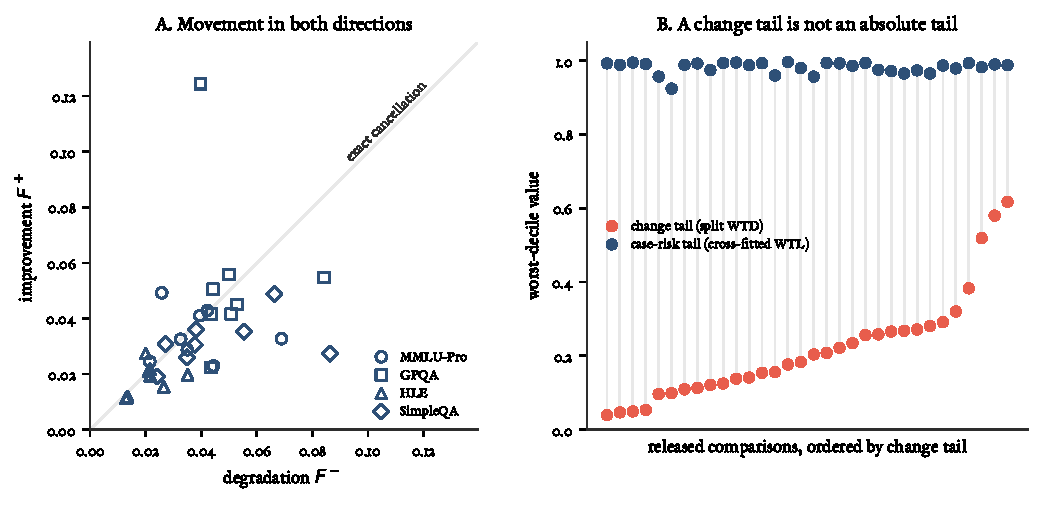
\includegraphics[width=0.96\linewidth]{analysis/outputs/hidden_distinctions.pdf}
\caption{Two distinctions the released aggregates conceal. (A) Directional components for the 32 comparisons. The diagonal is exact cancellation, where improvement and degradation are equal and the signed change is zero; distance from the origin is how far items moved, and distance from the diagonal is how much of that movement survived aggregation. (B) The change tail and the absolute case-risk tail for the same comparisons, ordered by the change tail. Both estimators use disjoint response information for selection and estimation, the split estimator for the change tail and cross-fitting for the case-risk tail, so the comparison isn't confounded by reuse of the same response noise. Neither thereby recovers an ideal latent population tail. Under a binary loss at these accuracies the case-risk tail is necessarily high; the point is that neither quantity determines the other or can substitute for it, not that they're statistically unrelated in every population.}\label{fig:hidden_distinctions}
\end{figure}

The null-referenced and split-tail procedures estimate different quantities. Split WTD exceeds the null-referenced value in 31 of the 32 released comparisons, by .0331 on average. Those comparisons share items within a benchmark and lineage across models, so the tally describes the fixed released set rather than 31 independent replications. Selecting and estimating the tail on the same responses inflates it: the raw estimate exceeds the split estimate by .0906 on average, ranging from .0330 to .1696. The null-referenced procedure subtracts a baseline-null expectation from a statistic selected and measured on all trials; it needn't remove bias under a nonnull effect. The split procedure selects items on one response half and measures their changes on the other, estimating the latent effect of a noisy-selected set rather than the ideal tail selected using unobserved latent item effects.

\begin{figure}[H]
\centering
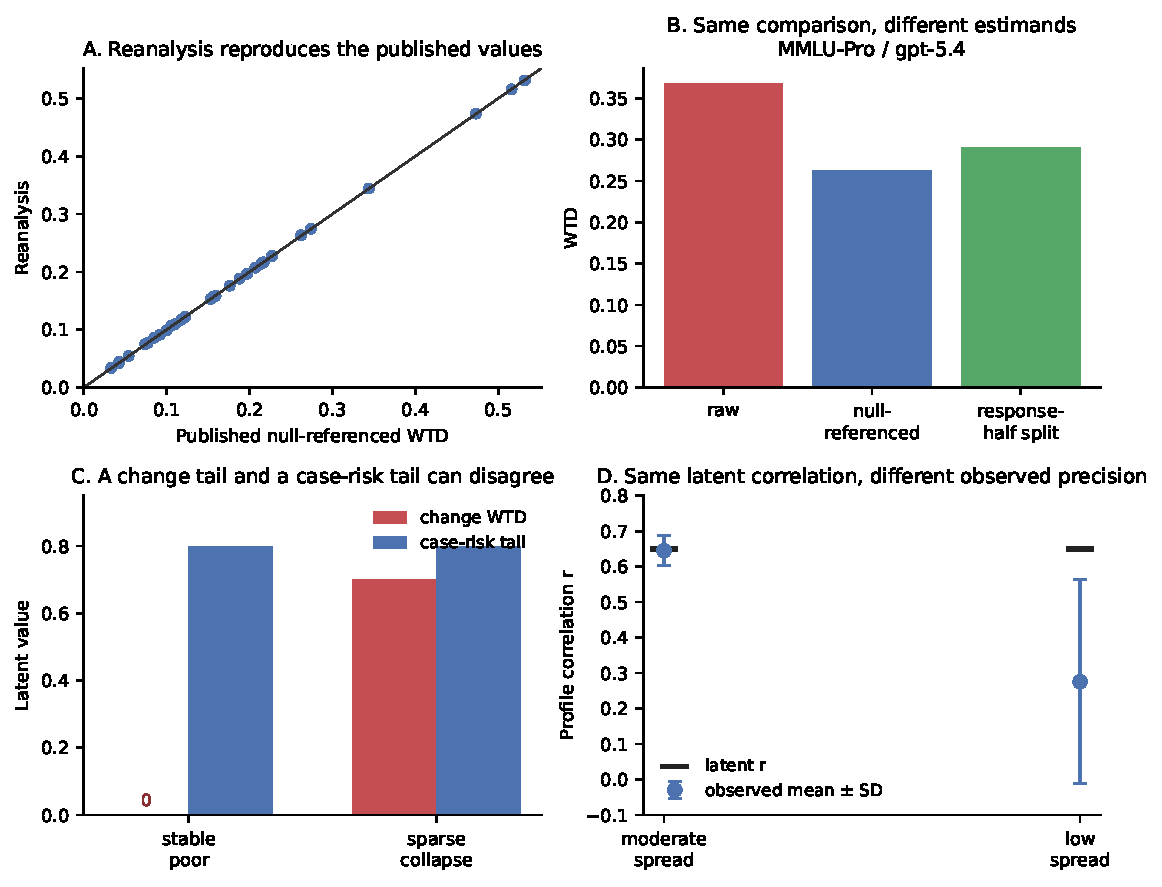
\includegraphics[width=0.94\linewidth]{analysis/outputs/section5_evidence.pdf}
\caption{Released-output reproduction and simulation checks. (A) Recomputed null-referenced WTD for all 32 comparisons against the rounded values reported by \textcite[4]{zhang2026illusionRobustness}. (B) Raw, null-referenced, and response-half split WTD for MMLU-Pro--gpt-5.4; the latter two target different estimands. (C) A simulation with stable, persistently poor performance on the same items has zero latent WTD but .80 worst-decile latent itemwise expected loss (case-risk WTL). (D) With ten domains and latent \(r=.65\), correlation estimation remains accurate at moderate profile spread but attenuates under low spread. Full settings and numerical outputs are in the empirical companion.}\label{fig:empirical_checks}
\end{figure}

\subsection{Known-Truth Checks}\label{ssec:known_truth}

Because simulations fix latent item probabilities, they make each estimator's target observable. Under a null effect, mean null-referenced INS, null-referenced WTD, and split WTD are .0033, .0039, and -.0018 against a truth of zero. Depending on the estimator, 31--56\% of the estimates are negative. Keeping those values untruncated is necessary for a zero-centred diagnostic.

In the sparse-collapse scenario, 10\% of items deteriorate by 55 percentage points while the remainder are unchanged. Null-referenced WTD averages .3445 against the ideal worst-decile effect of .5500 selected from the latent truth. Split WTD averages .4514 against a true mean of .4550 for the sets selected on noisy response halves, a bias of -.0036. Cross-fitting nearly removes reuse bias for its selected-set estimand, which differs from the ideal latent-tail estimand. Reports should state which tail they estimate.

In the stable-poor scenario, the same low-performing items have unchanged response probabilities across conditions, so latent WTD is zero. Their worst-decile latent itemwise expected loss is .80, the case-risk WTL. The tail of realized binary errors is a different estimand. Cross-fitted WTD and case-risk WTL are .0013 and .7911. A change tail and an absolute case-risk tail can disagree even without sampling error; the disagreement reflects their definitions.

The item bootstrap needs its own known-truth check, because a tail interval invites a reading it can't support. With 500 items, 20 trials per condition, and heterogeneous latent effects, 95\% item-bootstrap intervals cover the population signed change in .94 of replicates and population INS in .93. For the raw worst-decile statistic at that trial count they cover in .92, the mild undercoverage typical of a tail functional. For the latent worst-decile effect they cover in .00. Selection on response noise raises the population raw statistic from .160 to .295 while the interval is .056 wide, so the two never meet. An item bootstrap quantifies item sampling; it doesn't correct selection, and the null-referenced and split estimates are what address that.

The final simulation returns to the profile-correlation caution in Section~\ref{ssec:profile_level}. With ten domains and latent \(r=.65\), moderate between-domain spread yields a mean observed \(r=.645\) and root-mean-square error .043. Holding the latent correlation fixed while reducing profile spread lowers the mean observed correlation to .275 and raises root-mean-square error to .472. Coverage of 95\% bootstrap intervals that resample both domains and within-domain items falls from .988 to .579 even as mean interval width increases from .249 to 1.111.

When the perturbed latent profile is flat, its true correlation is undefined, but finite samples produce correlations with standard deviation .324. Reports should accompany \(r\) with the raw profiles and their spreads.

The reanalysis verifies the calculations on 32 fixed comparisons, and the simulations establish conditional estimator behaviour under their specified designs. Neither tests any inferential relation in Table~\ref{tab:projection_relations}; each requires a separate empirical design matched to the declared target, as Section~\ref{sec:validation} sets out. For the legal example, the results show why a developer should retain item changes and absolute failures rather than publish only a mean. They contain no research requests, legal-database searches, cited memos, or lawyer reviews, so they provide no estimate of performance on the firm's task.

\section{Testing Declared Projections}\label{sec:validation}

Once the observed outputs and the unobserved cases claimed are both stated, each extension needs evidence that tests the relevant difference. Evidence about benchmark content, how answers were produced, score structure, comparability across systems, out-of-sample prediction, causal explanation, and consequences in use supports different premises in the validity argument.

Predictive claims make the choice of holdout unit easiest to see, so they come first. The remaining subsections ask when an aggregate has a coherent interpretation, whether CHC-based interpretations transfer to AI systems, and what additional observations and value judgments a decision requires.

\subsection{Predictive Projection: Match the Statistical Design to the Claim}\label{ssec:matching}

For a predictive projection, each row of the analysis should represent the independent unit named by the claim. To extend from sampled to unsampled requests of the same eligible kinds, keep complete client-file clusters out of development. To extend from employment-law requests to tax research, sample tax requests rather than adding more employment files. To claim robustness to a new input alteration, keep one whole alteration type, such as injected topically similar cases, out of tuning. To claim transfer to another system, evaluate a different build or lineage; repeated drafts from one build aren't new systems. To claim transfer to another office, run the task and review procedure there, not merely with another lawyer from the first office. To predict later performance, use a chronological holdout. Response replicates estimate variation within a request--condition pairing; they don't multiply the number of requests, systems, alteration types, or periods.

Let \(u\) index the independent unit appropriate to a declared projection, \(Y_u\) the external outcome, and \(\mathbf X_u\) a preregistered set of predictors constructed without \(Y_u\). The unit depends on the claim. To test whether benchmark profiles predict legal-research performance across systems, \(u\) must index genuinely distinct builds or lineages, \(\mathbf X_u\) must contain each system's benchmark profile, and \(Y_u\) must be that system's defect rate on the same held-out research requests. With only one frozen assistant, its benchmark profile is constant across requests and can't predict which request will fail. A request-level model instead needs predictors that vary by request, such as request type, the number and age of retrieved authorities, conflicting appellate treatment, or the presence of the registered corpus alteration. Compare a simple model \(h_0\), such as the equal-domain benchmark average in the system-level study or the overall defect rate in the request-level study, with a richer model \(h_1(\mathbf X_u)\). Under a target prediction loss \(\mathcal L_T\), which scores forecasts of \(Y_u\) and is distinct from the item loss \(\ell^{(T)}\) of Section~\ref{ssec:wtl}, the relevant increment is
\[
\Delta_T
=\operatorname{E}_{\mathrm{holdout}}\!
\left[\mathcal L_T\{Y,h_0\}
      -\mathcal L_T\{Y,h_1(\mathbf X)\}\right].
\]
A positive estimate with decision-relevant uncertainty supports added predictive value within that holdout population. It doesn't establish transport to another population.

Shared baseline observations make perturbation comparisons dependent; related versions share lineage; and granular predictors are estimated with error. When many comparisons predict outcomes for few independent systems, analysts may need to constrain the fitted model or reduce the number of predictors. Models for repeated measurements can address dependence, hierarchical models can share information across groups, and methods for predictors measured with error can represent uncertainty in those predictors. Reports should state the observational row, dependence model, predictor construction, and final holdout.

For the firm's authorization decision, prompt development, rubric revision, and any predictive-model fitting use the older closed files and the alteration types assigned to development. The final block contains later client-file clusters and an alteration type not used in tuning. The defect definitions, \(\tau\), tail fraction, request-level predictors, and model tuning are fixed before that block is opened. Its results can estimate the larger of the two request-type case-risk tails for the frozen assistant. One such test can't calibrate a forecast of the next model build.

Forecasting the tail for a future build requires several earlier builds or work periods evaluated under a comparable protocol. A model of the event that the larger request-type tail exceeds \(\tau\) also requires enough build-level units to calibrate and score that event probability. Repeated requests from one build supply a more precise estimate of that build's tail; they don't create the build-level history needed to forecast another one. A model of request-level defect risk, a model of realized downstream loss, and a model of future tail exceedance are distinct predictive objects.

Incremental predictive value, estimation of the tail, and performance of the policy chosen from that evidence are three separate judgments. The final holdout is evaluated under the registered support, defeat, and inconclusive rules. Those rules should refer to the estimated defect tail, the red-line outcome, uncertainty, and \(\tau\), not merely to whether one interval endpoint crosses a number. The report should retain the continuous estimate; a policy may still use a boundary when the costs of false authorization and false rejection justify it. Too few independent client-file clusters, too few builds for a build-level forecast, or too few red-line events to estimate their rate can leave the claim unresolved rather than show that transfer failed. A defeated two-request-type claim moves only to its prespecified narrower test; it isn't repaired by selecting the requests that happened to pass.

\subsection{Commensurability, Compensability, and Projectibility}\label{ssec:score_model}

Predictive usefulness doesn't by itself make a collection of component scores a coherent aggregate. Aggregation introduces three separate questions. \term{Commensurability} asks whether differences on the components share a scale that makes addition interpretable. \term{Compensability} asks whether the substitutions permitted by the aggregate are acceptable for the intended interpretation or use. \term{Projectibility} asks whether the resulting score supports the declared target claim beyond the construction sample. The developer can add normalized legal-reasoning and quantitative scores, but the arithmetic doesn't show that a one-unit difference means the same thing on both components. Nor does a gain on quantitative questions compensate for a memo whose citation doesn't resolve or whose cited passage says something else. \Textcite[745--747]{messick1995Validity} treats the choice between compensatory totals, profiles, and minimum requirements as part of asking whether a score's structure matches its intended interpretation. Because a linear factor model of the kind underlying CHC and g builds in compensation \citep[632]{carroll1993human}, reading the total as a measure commits the interpretation to substitutions over stated score ranges even when the proposed use imposes a bottleneck or red-line requirement.

A monotone score such as
\[
S_T=\sum_{g=1}^{G}w_g^{(T)}a_{g0},
\qquad
w_g^{(T)}\geq0,\quad \sum_gw_g^{(T)}=1
\]
retains an ordinary direction: more of each component can't lower the total. It also encodes substitution among domains over the stated score ranges. Mapping heterogeneous scores to \([0,1]\) doesn't establish that equal differences have equal meaning or that those substitutions are acceptable. In a value model, the weights represent range-dependent tradeoffs rather than context-free domain importance \citep{KeeneyRaiffa1993}.

A predictive model fitted at an appropriate independent unit may legitimately use negative conditional coefficients, interactions, nonlinearities, or redundant predictors. Those coefficients needn't express value tradeoffs. An aggregate offered for interpretation, by contrast, shouldn't separately weight algebraically dependent quantities such as \(L\), INS, \(F^+\), and \(F^-\), because the redundancy obscures the effective coefficients on positive and negative change. WTD is bounded by the same components and coincides with \(-L\) at \(q=1\). Behavioural descriptions and target-conditioned risk shouldn't enter one interpretable total at all (Section~\ref{ssec:no_scalar}). Equal-domain weighting remains a useful descriptive and predictive baseline because it's transparent and difficult to tune, but equal nominal weights needn't make equal statistical contributions when domain variances and covariances differ \citep[305--308]{brennan2001generalizability}.

Each interpretation or use of the developer's total requires a different body of evidence. Treating it as a measure requires evidence that its tasks cover the intended domain, responses engage the relevant processes, score structure matches the construct, and scores remain comparable across systems. The evidence set is claim-specific, and omission of a potentially relevant basis needs justification \citep[744, 747]{messick1995Validity}. Treating the total as a predictive index requires target-matched out-of-sample performance. A causal explanation requires process evidence and interventions against plausible rival routes where access and the study design permit them. Removing a component and observing an effect establishes dependence over the tested levels; it doesn't by itself identify an internal representation or a corrective mechanism. Using the score in a release rule additionally requires defensible value scales, distributional tradeoffs, feasible alternatives, and evidence about decision performance.

Some accounts impose a stronger condition before calling an index a measure. \Textcite{borsboom2004conceptValidity} require variation in the measured attribute to cause variation in the score. If a study across several independent systems found that the total predicted the registered defect rate on held-out research requests, the firm might use it as a predictive input within that tested system population. That result still wouldn't show that the total measures a causally efficacious AGI attribute.

\subsection{Measurement Interpretation: CHC and Comparability}\label{ssec:chc_scope}

CHC theory \citep{carroll1993human,mcgrew2009chc,schneider2018chc} can enter AI evaluation in four roles. A taxonomy organizes content. A factor structure records which task scores vary together in a declared system population. A predictive input forecasts external outcomes. A functional or causal interpretation explains dependence. Evidence for one role doesn't establish the next. The framework proposed by \textcite{hendrycks2025agi} principally supplies the first; the other claims require additional study. In the running example, a CHC-organized profile can show which labelled domains supplied the battery's legal, verbal, or quantitative questions. It doesn't show that the assistant can retrieve the current controlling case, that its citation failures reflect a corresponding latent ability, that the same score covariance appears across model--retrieval builds, or that the profile predicts defects on the firm's held-out requests.

A distinction from cognitive measurement clarifies why these roles have to remain separate. \Textcite[179--181, 195--196]{embretson1983construct} distinguishes \term{construct representation}, the claim that specified processes, strategies, and knowledge stores underlie item responses, from \term{nomothetic span}, the score's network of relations with measures, criteria, groups, and tasks. Either can be strong while the other is weak.

Projectibility is assessed separately for each of these claims (Section~\ref{sec:projection}). A process model, a strong construct representation, doesn't itself establish external reach; and predictive success, a strong nomothetic span, doesn't show that the proposed process generated the score. For scores derived from factor models, too, validity is relative to a purpose and depends on analysis of both test and criterion tasks \citep[693]{carroll1993human}.

In factor analysis, a \term{loading} records how strongly a task score is associated with an inferred factor; a \term{positive manifold} is widespread positive correlation among task scores; and a \term{general factor} is a latent dimension introduced to account for much of that shared variation. These terms describe features of score covariation and of models fitted to it in a declared task and system population. They don't by themselves identify a system's internal capacities or establish that the same relations will hold in another population or in a system that adds retrieval, tools, and human review.

Task performances are observed, while broad and general abilities are inferred from their relations. Carrying human patterns of loadings or the positive manifold to artificial systems therefore requires evidence from the relevant artificial-system population. Even where a similar factor structure appears, the rule for combining abilities remains a separate choice: a target may permit additive compensation, impose minimum requirements, treat one domain as a bottleneck, or posit a causal chain in which one ability enables another. The firm's rule doesn't permit a high quantitative score, or strong performance on one request type, to offset an unresolvable citation on another. That noncompensatory decision rule needn't match the factor model that best summarizes covariance in the developer's test population.

Across 591 nominally distinct models and 12 tests, \textcite[4--5]{ilicGignac2024cognitiveCapabilities} find a positive manifold and a strong general factor. Their proposed hierarchy of four narrower factors beneath that general factor couldn't be interpreted; the narrower structure supported by their data combines knowledge with reading and writing. The largely verbal task set and the difficulty of identifying independent models also limit the result \citep[7--9]{ilicGignac2024cognitiveCapabilities}. The study supports a general factor for that sampled population of models and tests. It doesn't establish the human CHC decomposition for other artificial-system populations or for systems that combine a model with retrieval, tools, and human review.

Descriptive profiles can be compared without claiming that they measure identical latent abilities. Interpreting profile differences as differences in the same abilities across systems requires evidence that items and score relations retain the same interpretation: a linking or invariance argument. Depending on the design, comparability can be probed through rubric checks, family-specific item analyses, tests of whether particular items behave differently across system families after accounting for broader performance, and models that test whether item or factor relations remain comparable across groups \citep{meredith1993measurementInvariance}. Comparability is addressed assumption by assumption. \Textcite{jung2026psychometric} give a direct illustration: across 17 language models, human psychometric instruments showed moderate reliability across item and prompt variations while their scores failed to align with, and sometimes ran opposite to, model behaviour on downstream tasks. For the firm, a direct linking test would ask whether systems with higher legal-reasoning scores make fewer registered citation and authority errors on the same held-out requests. A shared label such as \mention{legal reasoning} supplies no answer.

Comparability isn't the only issue. The AGI label and the selection of domains also define which performances count as valuable. Content standards and score thresholds themselves need validation: higher score levels should reflect increasing complexity in the intended attribute rather than difficulty introduced by something outside it \citep[6]{messick1995standardsValidity}. Claiming that two systems meet the same standard presupposes comparability even when they aren't directly ranked \citep[7]{messick1995standardsValidity}. Once such a score informs action, the value choices become more explicit.

\subsection{Decision Use}\label{ssec:decision_use}

Decision framing specifies objectives, affected parties, consequences, feasible alternatives, preferences and tradeoffs, and hard constraints before a score is used to compare policies \citep{KeeneyRaiffa1993}. The firm has at least four policies to compare: no assistant, assistant-generated search suggestions, draft memos with line-by-line citation verification, and broader drafting with a lighter check. The firm, not the developer, has authority to decide which is permitted, and a numerical loss can represent its stated preferences but can't choose them. A nonresolving citation caught in the first review has a different consequence from the same citation sent to a client or relied on in court.

WTL averages a selected tail of case risks or realized losses under a declared sampling measure; neither form automatically shows who bears the consequences. The firm should therefore keep at least four records separate: defects in the generated draft, defects caught by the reviewing lawyer, defects remaining in the final memo, and defects that reach a client or court. It should also report results by request type and, where relevant, by the lawyers and client groups exposed to the system. The held-out defect score is only a surrogate for advice quality, delay, expense, or litigation consequences. Linking it to those outcomes requires shadow use and continuing incident and outcome records.

Pooling termination-clause and reasonable-notice requests requires a loss with the same meaning in both groups; pooling effects on clients, lawyers, and courts additionally requires a defensible rule for trading one party's loss against another's \citep{KeeneyRaiffa1993}. Calibration can't supply either rule. Constraining the larger of the two request-type tails prevents the more common or easier requests from compensating for the other type, but it still averages within the selected tail. The separate red-line rule does the work when no tradeoff is acceptable, as with an invented or unresolvable authority.

The firm needn't reduce all evidence to one number. A decision table can compare the policies on those records, lawyer time, and red-line incidents by request type, eliminating any that is no better on any dimension. It may also use hard constraints or a calibrated prediction model, but those structures answer different questions. A rule may combine a predicted defect rate with a case-risk or realized-loss WTL that the mean can't override; it must say whether the limit applies to the pooled requests, each type, or their maximum. Section~\ref{ssec:known_truth} gives a known-truth case in which the mean and change tail are stable while the case-risk tail is high. Imprecise evidence can't support broad authorization, though it may support search-suggestion use, mandatory review, or no use.

Observed consequences prompt at least three questions. If the assistant repeatedly omits recent appellate authority, the tested content may underrepresent the research task. If harmless document order changes move the score, the score may contain variation irrelevant to the claimed ability. If outputs pass the rubric but increase review time or allow an unsupported proposition into advice, the score may lack utility for the proposed policy. The firm may also reject a policy for distributive or ethical reasons even when prediction is accurate. These diagnoses can overlap, and favourable consequences can't rescue an invalid interpretation \citep[746--749]{messick1995Validity}. Accurate prediction of pooled loss likewise doesn't justify how a policy trades losses across clients, lawyers, courts, or third parties.

Decision evidence is comparative. The firm's mandatory-review policy should be assessed against no assistant, search suggestions only, and any lighter review policy using the same outcomes: lawyer time, pre- and post-review defects, red-line incidents, and what reaches clients or courts. The comparison exposes the value commitments in the rule \citep[748]{messick1995Validity}. Monitoring or authorization thresholds should be calibrated against those observed outcomes, not borrowed from the benchmark scale.

\section{Procedure and Limits}\label{sec:workflow}

The procedure begins with a sentence that can be contradicted by data and with a frozen description of the object tested. A claim about the benchmarked base model, a claim about the model connected to a legal database, and a claim about the final memo after lawyer review concern three different systems. The record must say which one each observation describes and what evidence is used to move from one to the next.

Responsibility is divided but not dissolved. Developers are responsible for evidence supporting the interpretations and uses they advertise, while deployers and decision-makers remain responsible for the choices they make; foreseeable consequences create shared obligations \citep[57--58]{kane2013validating}. A developer can publish the tested build and lineage, benchmark items and template clusters, prompts, scorers, item-level outputs, repeated-response design, registered alterations, uncertainty, and failures the evaluation didn't examine. Those observations remain conditional on the developer's item sample, scoring rule, and tested configuration.

A frontier developer can't know which employment-law questions a particular firm receives, which legal database it licenses, how its lawyers review citations, or what alternatives and consequences it faces. That limit narrows the developer's claim; it doesn't make task-specific testing optional. The firm must define the eligible requests, freeze the complete assistant, prepare or identify reference answers, sample its own work, record review and exposure, and compare the policies it can actually adopt \citep[744]{messick1995Validity}.

Most firms won't run the fullest version, and the framework doesn't require it. The firm can lean on the developer's published characterization and any independent evaluation for the item-level results, tails, and estimator diagnostics. Its own study can stay light: a modest audit of closed matters scored by the reviewing lawyer against the authorities already on file, a shadow phase that runs the assistant beside ordinary research without letting it determine the memo sent onward, and incident logging, rather than two blind reviewers preparing fresh reference answers and a bootstrapped tail. That lighter evidence won't establish a tail bound, but it can warrant mandatory line-by-line review on the two request types as a narrow, conservative authorization, widened as evidence accumulates and reopened after a model update, index change, revised prompt, new request type, or changed review procedure. Independent studies and data from another office may contribute only when the relevant task, system, and review differences are recorded. Thin evidence buys a narrow claim and a cautious policy, not a stronger verbal assurance.

\subsection{Operational Sequence}\label{ssec:workflow_sequence}

Most behavioural and predictive parts of the framework can be implemented without model internals. Measurement and causal claims may require process records or interventions that external evaluators can't obtain. The operational sequence is:

\begin{enumerate}
\item \textbf{Write one falsifiable claim.} Name the source observations, the unobserved cases to which they are being extended, the exact system, and the proposed use. Replace \mention{legal work} with an inclusion rule such as the two employment-law request types above, and replace \mention{the model} with a build, retrieval index, prompt stack, and review procedure. Register the support, defeat, inconclusive, and fallback conditions before examining confirmatory data.
\item \textbf{Turn every population noun into a column or sampling rule.} Record system lineage, client-file cluster, request and template type, alteration, lawyer and office, whether the output remained internal, entered client advice, or reached a filing; output replicate, scorer, pre- or post-review status, and date. State which levels are fixed, which are sampled, which combine, and which are nested. If a proposed facet can't be recorded or sampled, say that the corresponding extension is unsupported.
\item \textbf{Fix what counts as success and what decision is being made.} Prepare reference answers without seeing outputs; define each defect and any cardinal loss; keep ordinal hazards as categories or constraints; fix the tail fraction, minimum count, group rule, and uncertainty analysis; and list the feasible policies and their costs. State which outcomes are red lines rather than allowing them to be offset by gains elsewhere.
\item \textbf{Separate development from confirmation at the right level.} Keep all requests from one client file together. Hold out whole templates for item generalization, external task types for extrapolation, alteration types for context transport, lineages for system transport, offices for site transport, and later periods for temporal claims. Data used to write prompts, choose predictors, set \(\tau\), or revise the rubric can't also confirm the resulting claim.
\item \textbf{Collect and preserve the observations.} Balance paired conditions and randomize order where possible. Retain request identifiers, raw outputs, retrieval and review records, scorer decisions, exclusions, missingness, and every split assignment. Score drafts and reviewed outputs separately when the claim concerns the human--system procedure.
\item \textbf{Report description and risk without substitution.} Publish the registered behavioural quantities and uncertainty, the raw domain profiles and spreads, and the paired item changes needed to audit cancellation. State whether nonlinear estimates are raw, null-referenced, split-sample, or cross-fitted and which estimand each targets. Report target-conditioned loss separately, identifying whether the tail orders conditional case risks or realized losses, the loss scale, target distribution, exposure, residual randomness, surrogate status, and any group-specific or noncompensatory constraints.
\item \textbf{Test the claimed extension, not a nearby one.} Match the independent unit and holdout to the claim; assess content, process, scoring, comparability, prediction, causation, and decision consequences only with evidence that bears on each. A composite claim may combine two studies when the cases reached by the first are those sampled by the second, the interface assumptions are compatible, dependence and effect modification are represented, and uncertainty is propagated. A succession of successful but differently scoped tests doesn't add up to a claim none of them stated.
\item \textbf{Maintain the record after authorization.} The developer's evidence card should give build provenance, evaluation design, prompts, scoring, item-level results, uncertainty, known failures, and update triggers. The firm's addendum should give the task rule, system configuration, reference-answer and review procedures, results on eligible requests, permitted policy, deviations, monitoring fields, and incidents. Reopen the argument after a material change in the model, retrieval source, prompt, task mix, reviewers, or observed outcomes.
\end{enumerate}

\subsection{Limitations}\label{sec:limitations}

The framework itself is untested against deployment outcomes. The reanalysis and simulations verify what the quantities distinguish, not that any of them predicts a target.

Repeated sampling and tail estimation can be expensive. Adaptive allocation may reduce cost but adds selection and dependence. Deterministic fixed-set reports avoid repetition cost while remaining silent about wider item or context populations. Group-conditional assessment may require sensitive data and enough exposure in each stratum; without them, the corresponding claim is limited and a pooled substitute isn't licensed.

The estimators carry their own limits. Null-referenced contrasts are diagnostics against a baseline-only simulation rather than general bias corrections, and split-sample or cross-fitted tail estimates target the selected set rather than the population tail.

A perturbation is informative only relative to a property expected to remain invariant. Task-irrelevant context is designed to preserve the answer; distribution shifts, tool changes, and component removal may change the task itself. The evaluator has to defend the comparison.

Tail membership and item effects may not transfer across models or versions. \Textcite[2, 4--6]{zhang2026illusionRobustness} report a mean cross-model correlation of .00 for per-item change and a mean Jaccard overlap of .09 for the most-affected decile on MMLU-Pro, making a common risk set across models or versions an empirical hypothesis.

\section{Conclusion}\label{sec:conclusion}

An aggregate can describe its construction sample without supporting a broader inference. Generalizing from those observations to a declared evaluation universe and extrapolating from that universe to other tasks, contexts, systems, or times are distinct inferential steps.

The paired-condition module distinguishes profile shape, signed level, two-sided item change and its directional components, worst-tail degradation, case-risk tails, and realized-loss tails. None is a universal proxy for the others: the declared target identifies distinctions that may need to be preserved, while matched evidence determines which earn a place in a target-specific report. An aggregate interpreted as a measure or used in a decision also has to earn a common scale and acceptable tradeoffs among its components.

The reanalysis shows a small average decline coexisting with a much larger change tail, and the simulations show a change tail of zero coexisting with a high case-risk tail. Both show that raw, null-referenced, and split-sample estimators target different objects. Neither shows that any quantity predicts an untested target.

Goodman's riddle shows why fit to source observations can't, by itself, determine which extension is warranted. Validity belongs to a proposed interpretation and use; within that argument, projectibility is the degree of warrant for a specified extension from observed to unobserved cases. The practical discipline is to replace broad nouns with inspectable commitments: the exact outputs observed, the rule admitting target cases, the frozen system, the unit of analysis, the variations covered, the dates, the scored failures, the available policies, the evidence split, and the result that would narrow or defeat the claim. The record should retain enough item-level resolution to check whether aggregation hid a distinction relevant to that claim.

A CHC taxonomy may organize benchmark content, but claims that AI scores exhibit its narrower factor structure, remain comparable across systems, support external prediction, or provide evidence of AGI require separate support. Measurement interpretations need a defensible account of the evidential bases they implicate; predictions need target-matched external tests; and causal explanations need process evidence and tests against rivals. Decisions also require defensible values, alternatives, institutional authority, and continuing scrutiny of consequences.

Developers should report exactly what their evaluations observed and what they didn't test. Deployers should supply the missing observations for their own use and monitor what happens after review and exposure. In the example, the developer's legal-reasoning score describes answers under the battery's prompts and materials. The firm's authorization argument instead depends on sampled research requests, independently prepared authority lists, citation and omission scores, lawyer-review records, the comparison among feasible policies, and incidents in use. Repeating or aggregating benchmark scores can't supply those observations. Open-ended AGI claims require more than accumulated coverage. Bounded empirical projections may be combined with substantive or formal reasons for extending them, but successful projections don't automatically compose into unrestricted generality. A warranted inference from an aggregate rests on a declared, revisable argument whose evidence matches the scope of each claim.

\clearpage

\appendix

\section{Deployment-facing tail definitions}\label{app:deployment_tails}

Section~\ref{ssec:target_risk} replaces the equally weighted finite-set tails with tails over the population a decision concerns. This appendix states that construction.

For a deployment-facing target \(T\), let \(J\sim P_T\) index a joint draw over every varying facet in scope, including system, task or episode, domain, perturbation family and realization, operator, affected-population stratum, and time. Let \(R\) collect response, scorer, and downstream-outcome randomness conditional on \(J\), let \(S_{JcR}\) be the realized score under condition \(c\), and let \(\ell^{(T)}_{JR}\in[0,1]\) be realized target loss. Define \(\delta_J=\operatorname{E}_R(S_{JpR}-S_{J0R}\mid J)\), \(D_J=-\delta_J\), and \(\mu^{(T)}_J=\operatorname{E}_R(\ell^{(T)}_{JR}\mid J)\).

With \(Q_{V,T}\) the quantile function of \(V\), which gives the cutoff at cumulative probability \(u\) under the indicated target distribution, define
\[
\operatorname{ES}^{+}_{q,T}(V)
=\frac{1}{q}\int_{1-q}^{1}Q_{V,T}(u)\,\mathrm du.
\]
The deployment-facing change tail and absolute-loss tails are
\[
\operatorname{WTD}_{q,T}=\operatorname{ES}^{+}_{q,T}(D_J),
\qquad
\wtl^{\mathrm{case}}_{q,T}=\operatorname{ES}^{+}_{q,T}(\mu^{(T)}_J),
\qquad
\wtl^{\mathrm{real}}_{q,T}=\operatorname{ES}^{+}_{q,T}(\ell^{(T)}_{JR}).
\]

The expected-shortfall functional orders probability mass rather than merely similar-looking benchmark items. When the distribution is discrete and the cutoff falls within a probability mass, the tail calculation includes only enough of that mass to reach the chosen fraction. The realized-loss measure integrates both \(P_T(J)\) and the conditional distribution of \(R\), so it generally differs from the tail of conditional case risks \(\mu^{(T)}_J\).

\clearpage

\printbibliography

\end{document}
